Même si la pluralité des approches musicales amène à l'éclatement d'une pratique notationnelle unique, la partition n'en reste pas moins \og un moyen pour le compositeur de penser sa musique, la décrire et la communiquer grâce à un système de représentation symbolique \fg \cite{bresson2008}.
En effet, le projet \textit{symbolist} (voir section \todo{ref vers section}), qui constitue le cadre du présent stage de recherche, a été impulsé par Jean Bresson et Rama Gottfried, dans l'optique d'offrir aux compositeurs de "musique multimédia" un outil informatique pour la spécification de leur propre notation.
Par conséquent, cette partie s'intéresse à la définition de la "musique multimédia" et expose les problématiques liées à son écriture.

\subsection{Définition}

La \emph{musique multimédia}, ou \emph{composition multimédia} (\textit{media composition} en anglais), est un expression employée par Rama Gottfried dans \cite{gottfried2017}; elle désigne une pratique qui englobe la simple composition musicale.
La suivante définition d'une telle musique est proposée au lecteur : la musique multimédia décrit une pratique compositionnelle et artistique, qui, par l'entremise de moyens et supports divers empruntés au domaine audiovisuel (instruments de musique, ordinateurs, installation physique…), se constitue en vecteur d'une expérience multisensorielle (sonore, visuelle, tactile…).

La distinction est faite entre la musique multimédia et la performance artistique, en ce que la première implique une dimension sonore et musicale récurrente lors de son exécution.

Comme illustration de la musique multimédia, un fragment de la partition de la pièce \textit{Fluoresce} (R. Gottfried, 2012) est présentée en figure \ref{fig:schemaInstallationFluoresce}.

\begin{figure}[H]
	\centering
	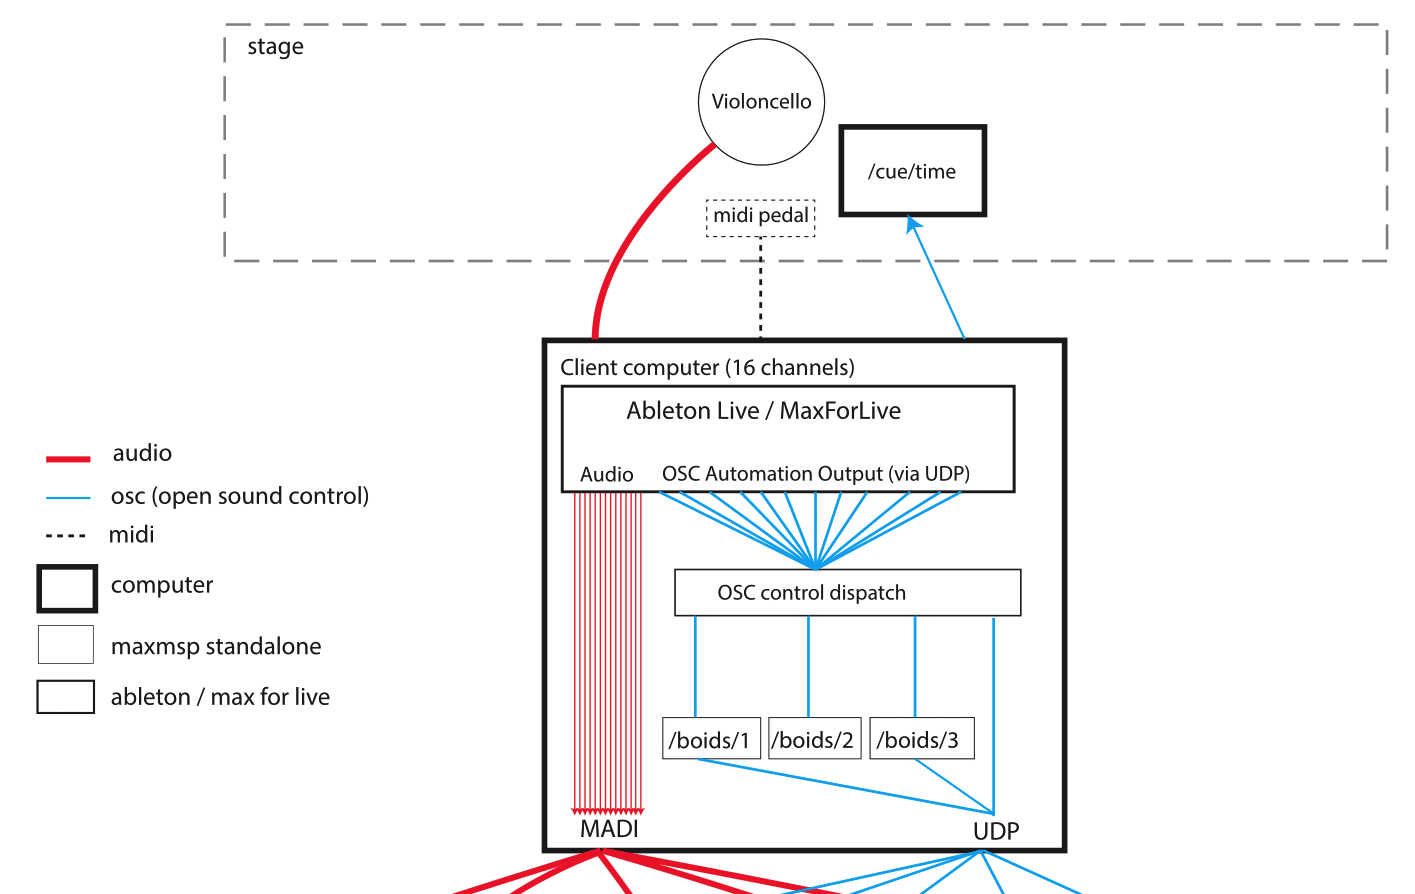
\includegraphics[keepaspectratio=true, width=\textwidth]{Notation/i/schemaInstallationFluoresce.png}
	\caption[Schéma de branchement pour la pièce \textit{Fluoresce} par Rama Gottfried]{Schéma de branchement pour la pièce \textit{Fluoresce} par Rama Gottfried}
	\label{fig:schemaInstallationFluoresce}			
\end{figure}
\begin{center}
\small \it Cette figure présente le schéma de câblage des différents éléments qui vont servir à l'exécution de la pièce. La performance fait intervenir un joueur de violoncelle (\textit{Violoncello}); le son produit par le violoncelle est capté et envoyé à un ordinateur (\textit{Client computer}) sur lequel est lancé la station audionumérique\footnote{Une station audionumérique (acronyme DAW, de l'anglais digital audio workstation) désigne une station de travail dédiée à l'audionumérique. C'est un ensemble d'outils électroniques, conçu pour enregistrer, éditer, manipuler, créer et lire des contenus audionumériques. -- Wikipédia} \textit{Ableton Live} associé au plugin \textit{MaxForLive}\footnote{MaxForLive est un plugin permettant l'intégration du logiciel Max/MSP à la station audionumérique Ableton Live. Voir plus loin pour plus de détails sur Max/MSP.}. Ableton Live va répartir le signal audio sur les systèmes WFS et HOA (\textit{Wave Field Synthesis} et \textit{High Order Ambisonics}\footnote{\textit{Wave Field Synthesis} et \textit{High Order Ambisonics} sont deux systèmes de diffusion de sons spatialisés basés sur l'utilisation d'un grand nombre d'enceintes.}) via la liaison MADI\footnote{MADI (Multichannel Audio Digital Interface) est une liaison audionumérique définissant un protocole capable d'embarquer 64 canaux audio simultanément}. Le plugin MaxForLive va s'occuper d'envoyer des messages OSC\footnote{Open Sound Controle. Protocole décrivant des messages sous forme d'urls. \textbf{Voir le chapitre} pour plus de détails.} \texttt{/boids/1}, \texttt{/boids/2} et \texttt{/boids/3} (directives de déclenchement d'effets sonores), via UDP, aux systèmes WFS et HOA. Le schéma de branchement complet est consultable en annexe \ref{sec:schemaInstallationFluoresceComplet} page~\pageref{sec:schemaInstallationFluoresceComplet}.
\end{center}

Cette pièce met bien en place des moyens audiovisuels (un violoncelle, des ordinateurs, et deux systèmes de diffusion sonore…) pour traduire une expérience musicale; ici l'expérience est purement sonore, il n'y a pas de dimension multisensorielle. La pièce \textit{Fluoresce} est un type de musique appelée "musique mixte", c'est à dire qui mélange instruments traditionnels et informatique.

Sur le schéma, un ordinateur sur scène envoie le message OSC \texttt{/cue/time} au \textit{Client computer}. Le message \texttt{/cue/time} transmet un référentiel temporel permettant la synchronisation entre le jeu du violoncelliste et le \textit{Client computer}. 
Dans le cas de musique mixte, la question de la synchronisation humain/machine et du suivi de partition est centrale (voir la section suivante). 
En effet, même si une pièce de musique multimédia peut se détacher de toutes notions de métrique, de mélodie et d'harmonie, elle ne peut se détacher de la temporalité des évènements qui la composent et qui nécessite un interaction synchrone entre les acteurs de la pièce. 


